\section{La Funcionalidad Estrella: Fail-Fast}

\subsection{Cancelando tempranamente}
\begin{frame}
    \frametitle{¿Qué pasa cuando una validación falla antes de que las otras terminen de ejecutar?}

    \begin{alertblock}{Reactive Basic: Sin fail-fast}
        \begin{itemize}[<+->]
            \item \texttt{allOf()} espera que TODAS las tareas terminen
            \item Sin cancelación → desperdicio de recursos
            \item ~570ms incluso si falla en 200ms
        \end{itemize}
    \end{alertblock}

    \onslide<+->
    \begin{exampleblock}{Reactive "Fixed": Fail-fast manual}
        \begin{itemize}[<+->]
            \item Se puede lograr $\ldots$ pero requiere lógica compleja
            \item \texttt{failFast.completeExceptionally()} + coordinación manual
        \end{itemize}
    \end{exampleblock}

    \onslide<+->
    \begin{block}{Structured: Fail-fast automático}
        \begin{itemize}[<+->]
            \item \texttt{StructuredTaskScope.open()} = fail-fast por defecto
            \item Cancelación automática en cascada
        \end{itemize}
    \end{block}

    \begin{center}
        \Large{\textcolor{red}{$\blacktriangleright$ La demo más importante...}}
    \end{center}
\end{frame}

\subsection{Por Qué Esto Importa}
\begin{frame}
    \begin{exampleblock}{Impacto en la Experiencia de Usuario}
        \begin{itemize}[<+->]
            \item \textbf{Falla rápido}: Reporta errores inmediatamente, mejor UX
            \item \textbf{Menor latencia} en casos de error
            \item \textbf{Feedback claro}: Usuario no espera innecesariamente
        \end{itemize}
    \end{exampleblock}

    \onslide<+->
    \begin{block}{Impacto en Recursos y Costos}
        \begin{itemize}[<+->]
            \item \textbf{Eficiencia}: Cancela trabajo innecesario automáticamente
            \item \textbf{Ahorro de CPU}: No procesa validaciones que no se usarán.
            \item \textbf{Menor carga}: Sistema responde más rápido en picos de errores
        \end{itemize}
    \end{block}

\end{frame}

\subsection{Ejemplo de mejora}
\begin{frame}
    \frametitle{Resumen de rendimiento: Éxito vs Fallo}

    \begin{columns}
        \column{0.48\textwidth}
        \onslide<+->
        \begin{exampleblock}{Caso Exitoso: Paridad}
            \begin{itemize}
                \item \textbf{Sin fallo temprano}: ~750ms
                \item \textbf{Con fallo temprano}: ~750ms
                \item \textbf{Resultado}: Mismo rendimiento
            \end{itemize}
        \end{exampleblock}

        \onslide<+->
        \begin{block}{¿Por qué iguales?}
            Ambos deben esperar que todas las validaciones terminen.
        \end{block}

        \column{0.48\textwidth}
        \onslide<+->
        \begin{alertblock}{Caso Fallido: Más Rápido}
            \begin{itemize}
                \item \textbf{Reactive}: ~750ms
                \item \textbf{Structured}: ~330ms
                \item \textbf{Mejora}: \textcolor{red}{\textbf{56\%}}
            \end{itemize}
        \end{alertblock}

        \onslide<+->
        \begin{block}{¿Por qué?}
            \begin{itemize}
                \item Sin fail fast: Esperar a que todas las validaciones terminen.
                \item Con fail fast: Cancela automáticamente cuando la primera falla.
            \end{itemize}
        \end{block}
    \end{columns}

    \vspace{1em}
\end{frame}
\begin{frame}
    \begin{center}
        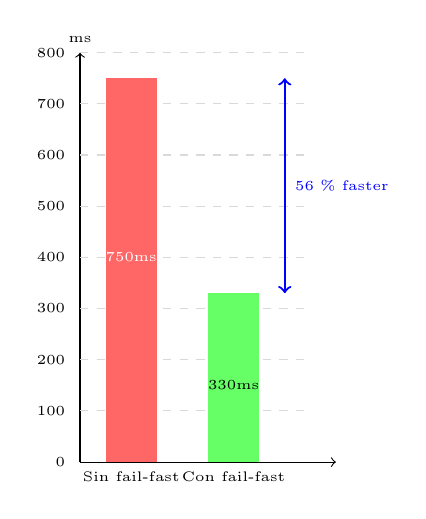
\begin{tikzpicture}[scale=0.65]
            % Y axis
            \draw[->] (0,0) -- (0,8) node[anchor=south] {\tiny ms};
            % X axis
            \draw[->] (0,0) -- (5,0);

            % Grid lines
            \foreach \y in {1,2,3,4,5,6,7,8}
            \draw[dashed, gray!30] (0,\y) -- (4.5,\y);

            % Y axis labels
            \node[anchor=east] at (-0.1,0) {\tiny 0};
            \node[anchor=east] at (-0.1,1) {\tiny 100};
            \node[anchor=east] at (-0.1,2) {\tiny 200};
            \node[anchor=east] at (-0.1,3) {\tiny 300};
            \node[anchor=east] at (-0.1,4) {\tiny 400};
            \node[anchor=east] at (-0.1,5) {\tiny 500};
            \node[anchor=east] at (-0.1,6) {\tiny 600};
            \node[anchor=east] at (-0.1,7) {\tiny 700};
            \node[anchor=east] at (-0.1,8) {\tiny 800};

            % Reactive bar (750ms ≈ 7.5 units)
            \fill[red!60] (0.5,0) rectangle (1.5,7.5);
            \node[anchor=north, font=\tiny] at (1,0) {Sin fail-fast};
            \node[font=\tiny, white] at (1,4) {750ms};

            % Structured bar (330ms ≈ 3.3 units)
            \fill[green!60] (2.5,0) rectangle (3.5,3.3);
            \node[anchor=north, font=\tiny] at (3,0) {Con fail-fast};
            \node[font=\tiny] at (3,1.5) {330ms};

            % Arrow showing difference
            \draw[<->, thick, blue] (4,3.3) -- (4,7.5) node[midway, right, font=\tiny] {56 \% faster};

        \end{tikzpicture}
    \end{center}

    \begin{exampleblock}{Conclusi\'on}
        Mejor experiencia del usuario y menor uso de recursos en casos de error. \\
        Misma eficiencia en casos de éxito.
    \end{exampleblock}
\end{frame}

